\section{Overview of state databases} \label{Overview of state databases}

\subsection{Databases implementing Andmejälgija}

\subsubsection{Digital Registry (Digiregistratuur)}
The Digital Registry demonstrates exemplary implementation of the Andmejälgija protocol. They provide very descriptive information about data access requests, making it clear to users why their data was accessed and by whom.

\subsubsection{Other databases implementing Andmejälgija}
\begin{itemize}
    \item Residence and Work Permit Register (Elamislubade ja töölubade register)
    \item Land Register (Kinnistusraamat)
    \item Professional Qualifications Register (Kutseregister)
    \item Taxpayers Register (Maksukohustuslaste register)
    \item Police Tactical Management Database (Politsei taktikalise juhtimise andmekogu)
    \item Agricultural Animals Register (Põllumajandusloomade register)
    \item Agricultural Subsidies and Land Blocks Register (Põllumajandustoetuste ja põllumassiivide register)
    \item Population Register (Rahvastikuregister)
    \item Prescription Centre (Retseptikeskus)
    \item Social Protection Information System (Sotsiaalkaitse infosusteem)
    \item Social Services and Benefits Register (Sotsiaalteenuste ja toetuste register)
    \item Labour Inspectorate Working Life Information System (Tööinspektsiooni tooelu infosusteem)
    \item Unemployment Insurance Database (Töötuskindlustuse andmekogu)
\end{itemize}

\subsection{Databases providing other form of data access tracking}

\subsubsection{E-File System (E-toimik)}
E-File System provides its own web-view for displaying requests made about the user, independent of the standard Andmejälgija protocol.
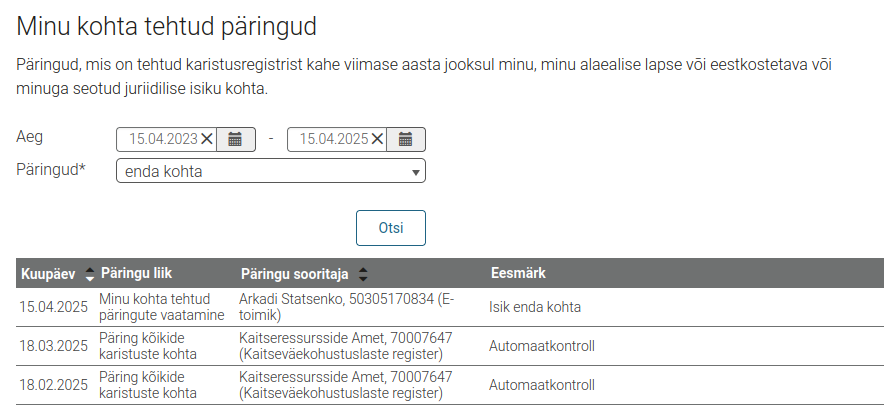
\includegraphics[width=450px]{english/figures/e-toimik.png}

\subsection{Databases not providing any kind of data access tracking}
\begin{itemize}
    \item Schengen Information System
    \item Border Control Database (Piirikontrolli andmekogu - PIKO)
    \item POLIS Information System (Infosusteem POLIS)
    \item Vehicle Registration Database (Liiklusregister)
    \item Court Information System (Kohtute infosüsteem - KIS)
    \item Employment register (Töötamise register (TÖR))

\end{itemize}


